In \autoref{s:Contribution-2-Motivation} we discuss how ... \hinttext{Explain how this chapter is structured. Make sure you cover all sections!} We summarize our discussion in \autoref{s:Contribution-2-Summary}.

\section{Motivation}
\label{s:Contribution-2-Motivation}

%\begin{longtable}{@{}l *{2}{rr}}
\begin{longtable}[h!]{@{}l *{2}{rr}}
\caption[Portrait Table, short caption]{Variables Correlation}
\label{t:correlation_table}
\\
%   
\toprule%


 {\bfseries Variable} & {\bfseries COD\textsubscript{D} } & {\bfseries COD\textsubscript{EQ}} & {\bfseries MLVSS}
\\

\cmidrule[0.4pt](r{0.125em}){1-1}%
\cmidrule[0.4pt](lr{0.125em}){2-4}%
%\cmidrule[0.4pt](lr{0.125em}){4-5}%
%\cmidrule[0.4pt](lr{0.125em}){5-6}%


  \endfirsthead

\endhead

        Flow\_to\_EQ & 0.14 & -0.14 & -0.025  \\ 
        BT\_C\_MLSS & 0.11 & -0.43 & 0.88  \\ 
        BT\_C\_MLVSS & 0.10 & -0.45 & 0.9  \\ 
        BT\_N\_MLSS & 0.10 & -0.44 & 0.88  \\ 
        BT\_N\_MLVSS & 0.10 & -0.44 & 0.88  \\ 
        D\_SS & 0.3 & 0.59 & -0.46  \\ 
        EQ\_N & 0.25 & 0.74 & -0.54  \\ 
        BT\_C\_N & 0.25 & 0.49 & -0.54  \\ 
        BT\_N\_N & 0.11 & 0.26 & -0.47  \\ 
        D\_N & 0.11 & 0.23 & -0.46  \\ 
        OxT\_pH & -0.12 & -0.33 & 0.27  \\ 
        EQ\_pH & -0.069 & 0.18 & -0.17  \\ 
        BT\_N\_pH & 0.057 & -0.045 & 0.083  \\ 
        D\_pH & 0.059 & -0.13 & 0.078  \\ 
        BT\_N\_DO & -0.1 & -0.37 & 0.14  \\ 
        BT\_C\_DO & -0.28 & -0.33 & 0.34  \\ 
        Clari\_DO & -0.17 & -0.43 & 0.27  \\ 
        ST\_COD & 0.22 & 0.63 & -0.44  \\ 
        D\_COD\_ON & 0.72 & 0.22 & 0.11  \\


\bottomrule

\end{longtable}
\autoref{t:correlation_table} presents the Pearson correlation of the three target variables this study covers.

\section{Major point 1}
\label{s:Contribution-2-Major-1}
Develop your idea! For example, discuss the axioms that underpin the inner workings of your algorithms.

\subsection{Minor idea 1}
\label{s:Contribution-2-Major-1-Minor-1}
Develop your idea! For example, explain how your algorithm actually works.

\begin{figure}[h]
\centering
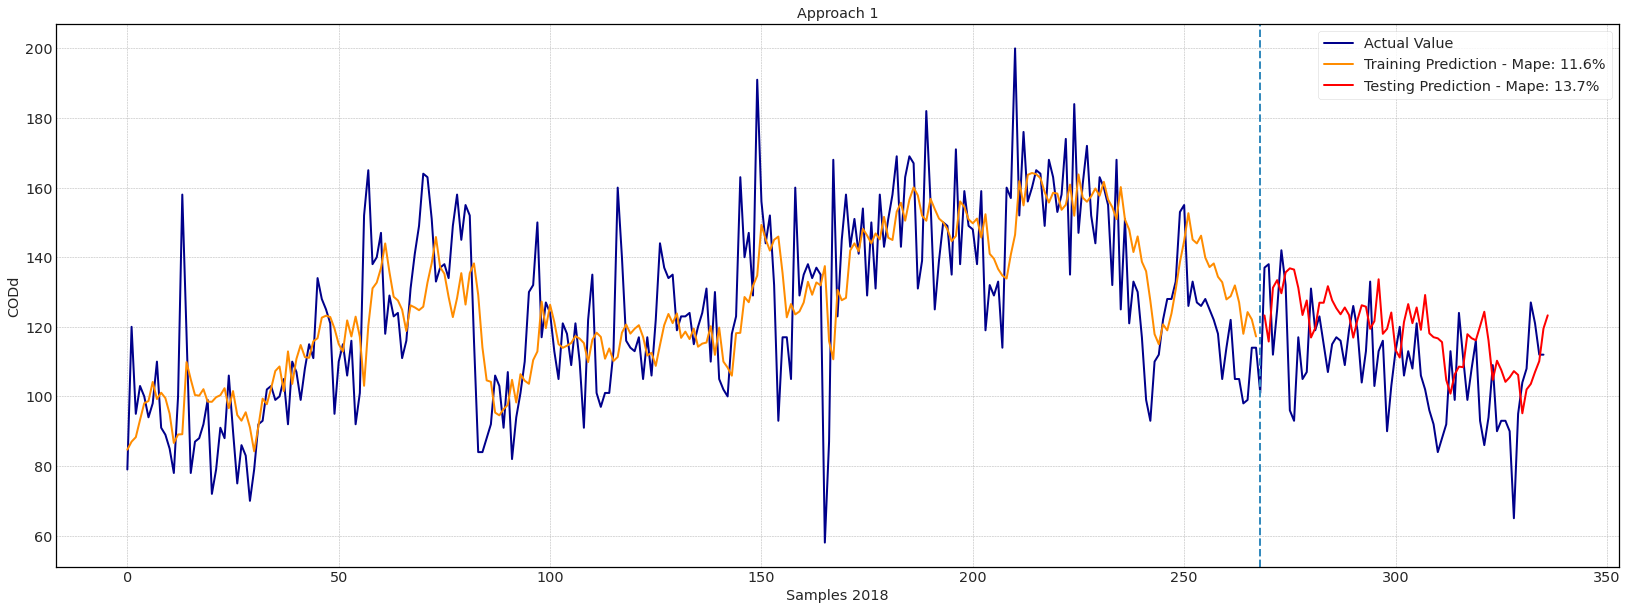
\includegraphics[width=\linewidth]{figures/Ch4/CODd-1.png}
\caption{Approach 1 - CODD}
\label{f:App1-codd}
\end{figure}

\begin{figure}[h]
\centering
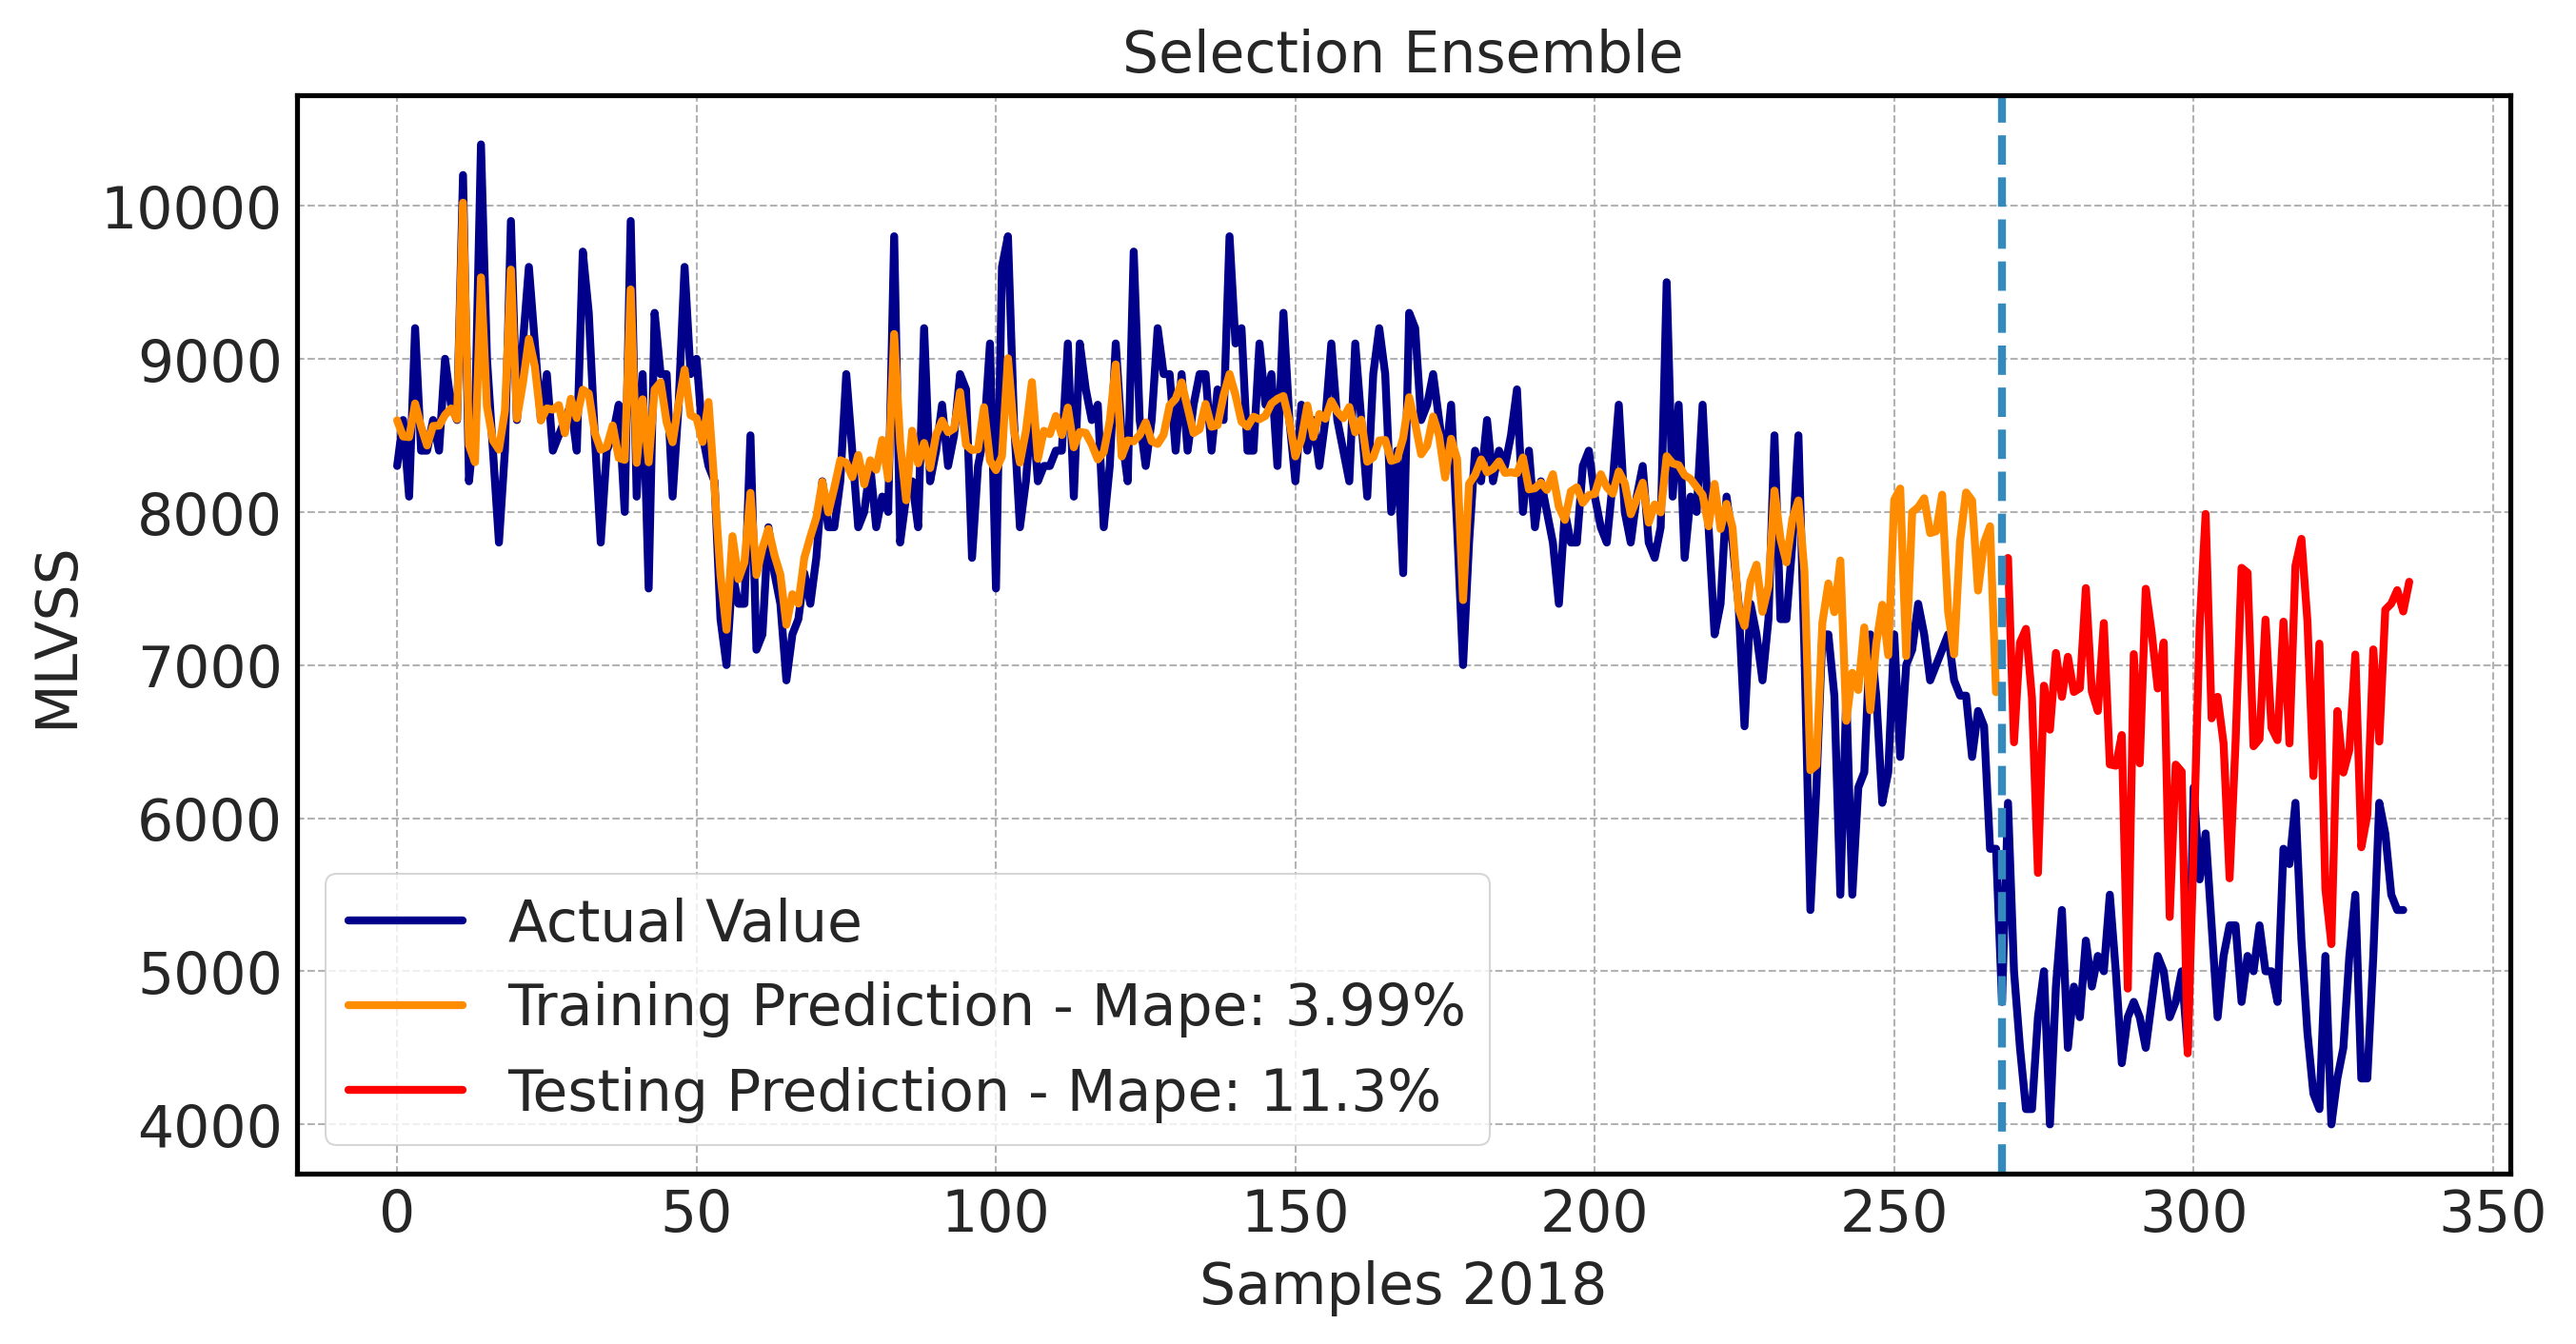
\includegraphics[width=\linewidth]{figures/test2.png}
\caption{Approach 1 - CODEQ}
\label{f:App1-codeq}
\end{figure}

\begin{figure}[h]
\centering
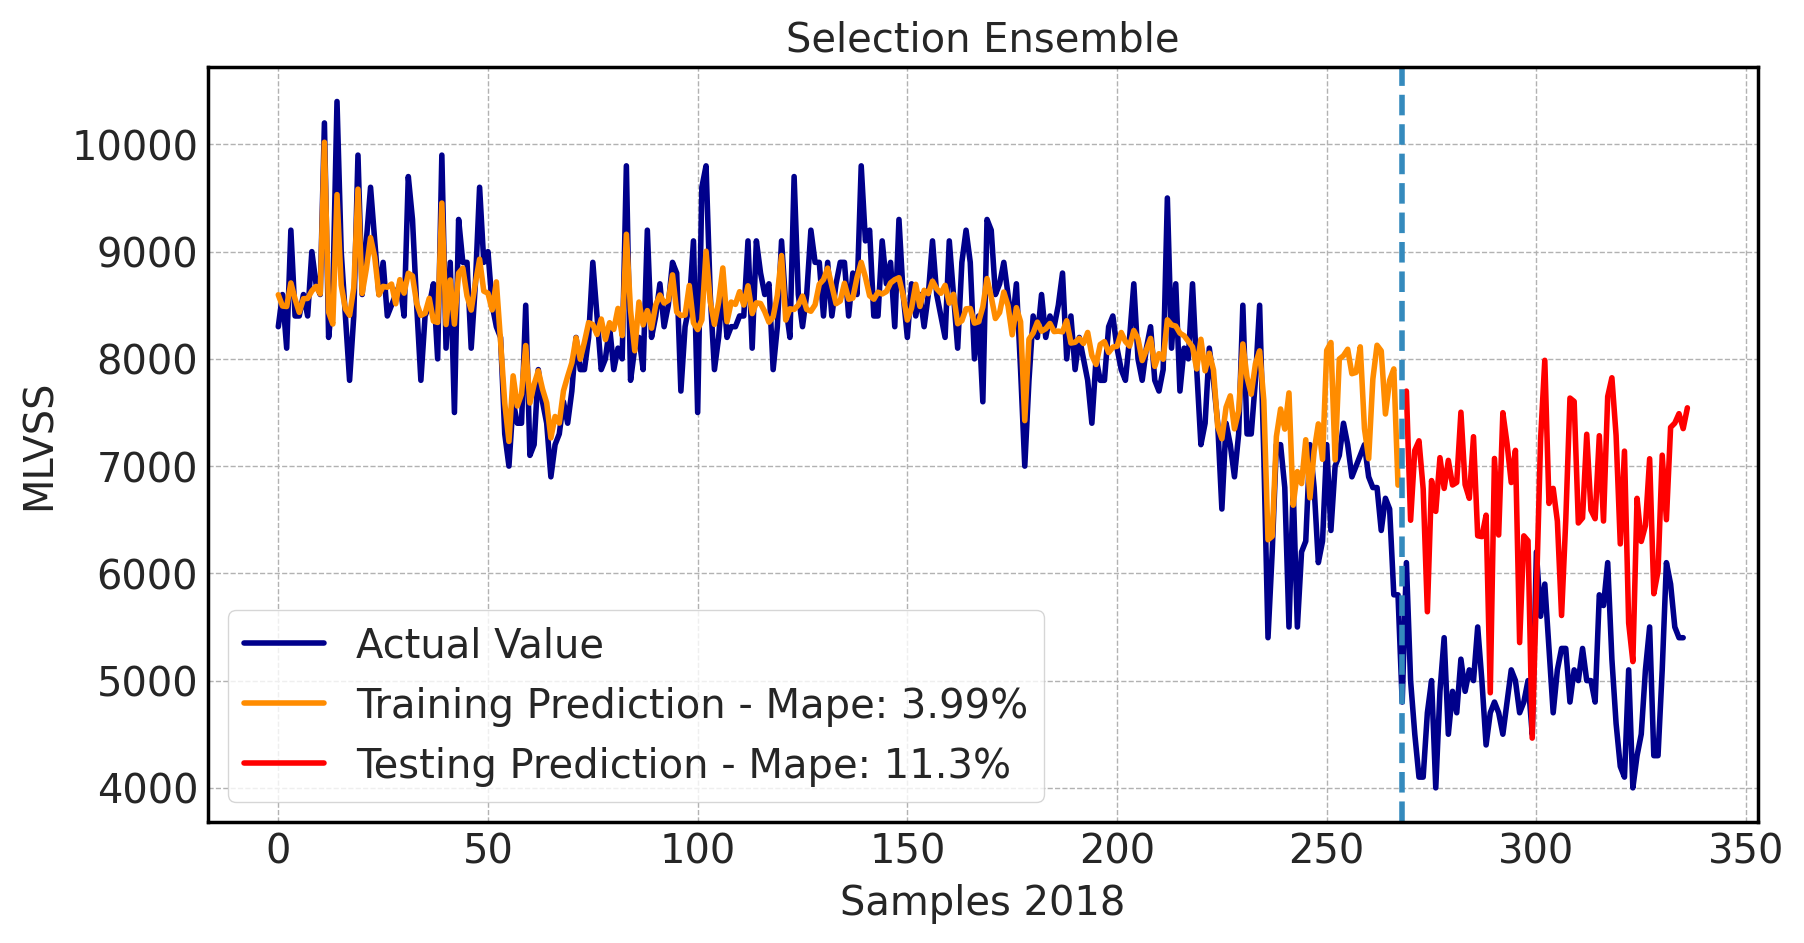
\includegraphics[width=\linewidth]{figures/test.png}
\caption{Approach 1 - MLVSS}
\label{f:App1-MLVSS}
\end{figure}

\subsection{Minor idea 2}
\label{s:Contribution-2-Major-1-Minor-2}
Develop your idea! For example, explain how the theoretical limits of your approach.

\begin{figure}[h]
\centering
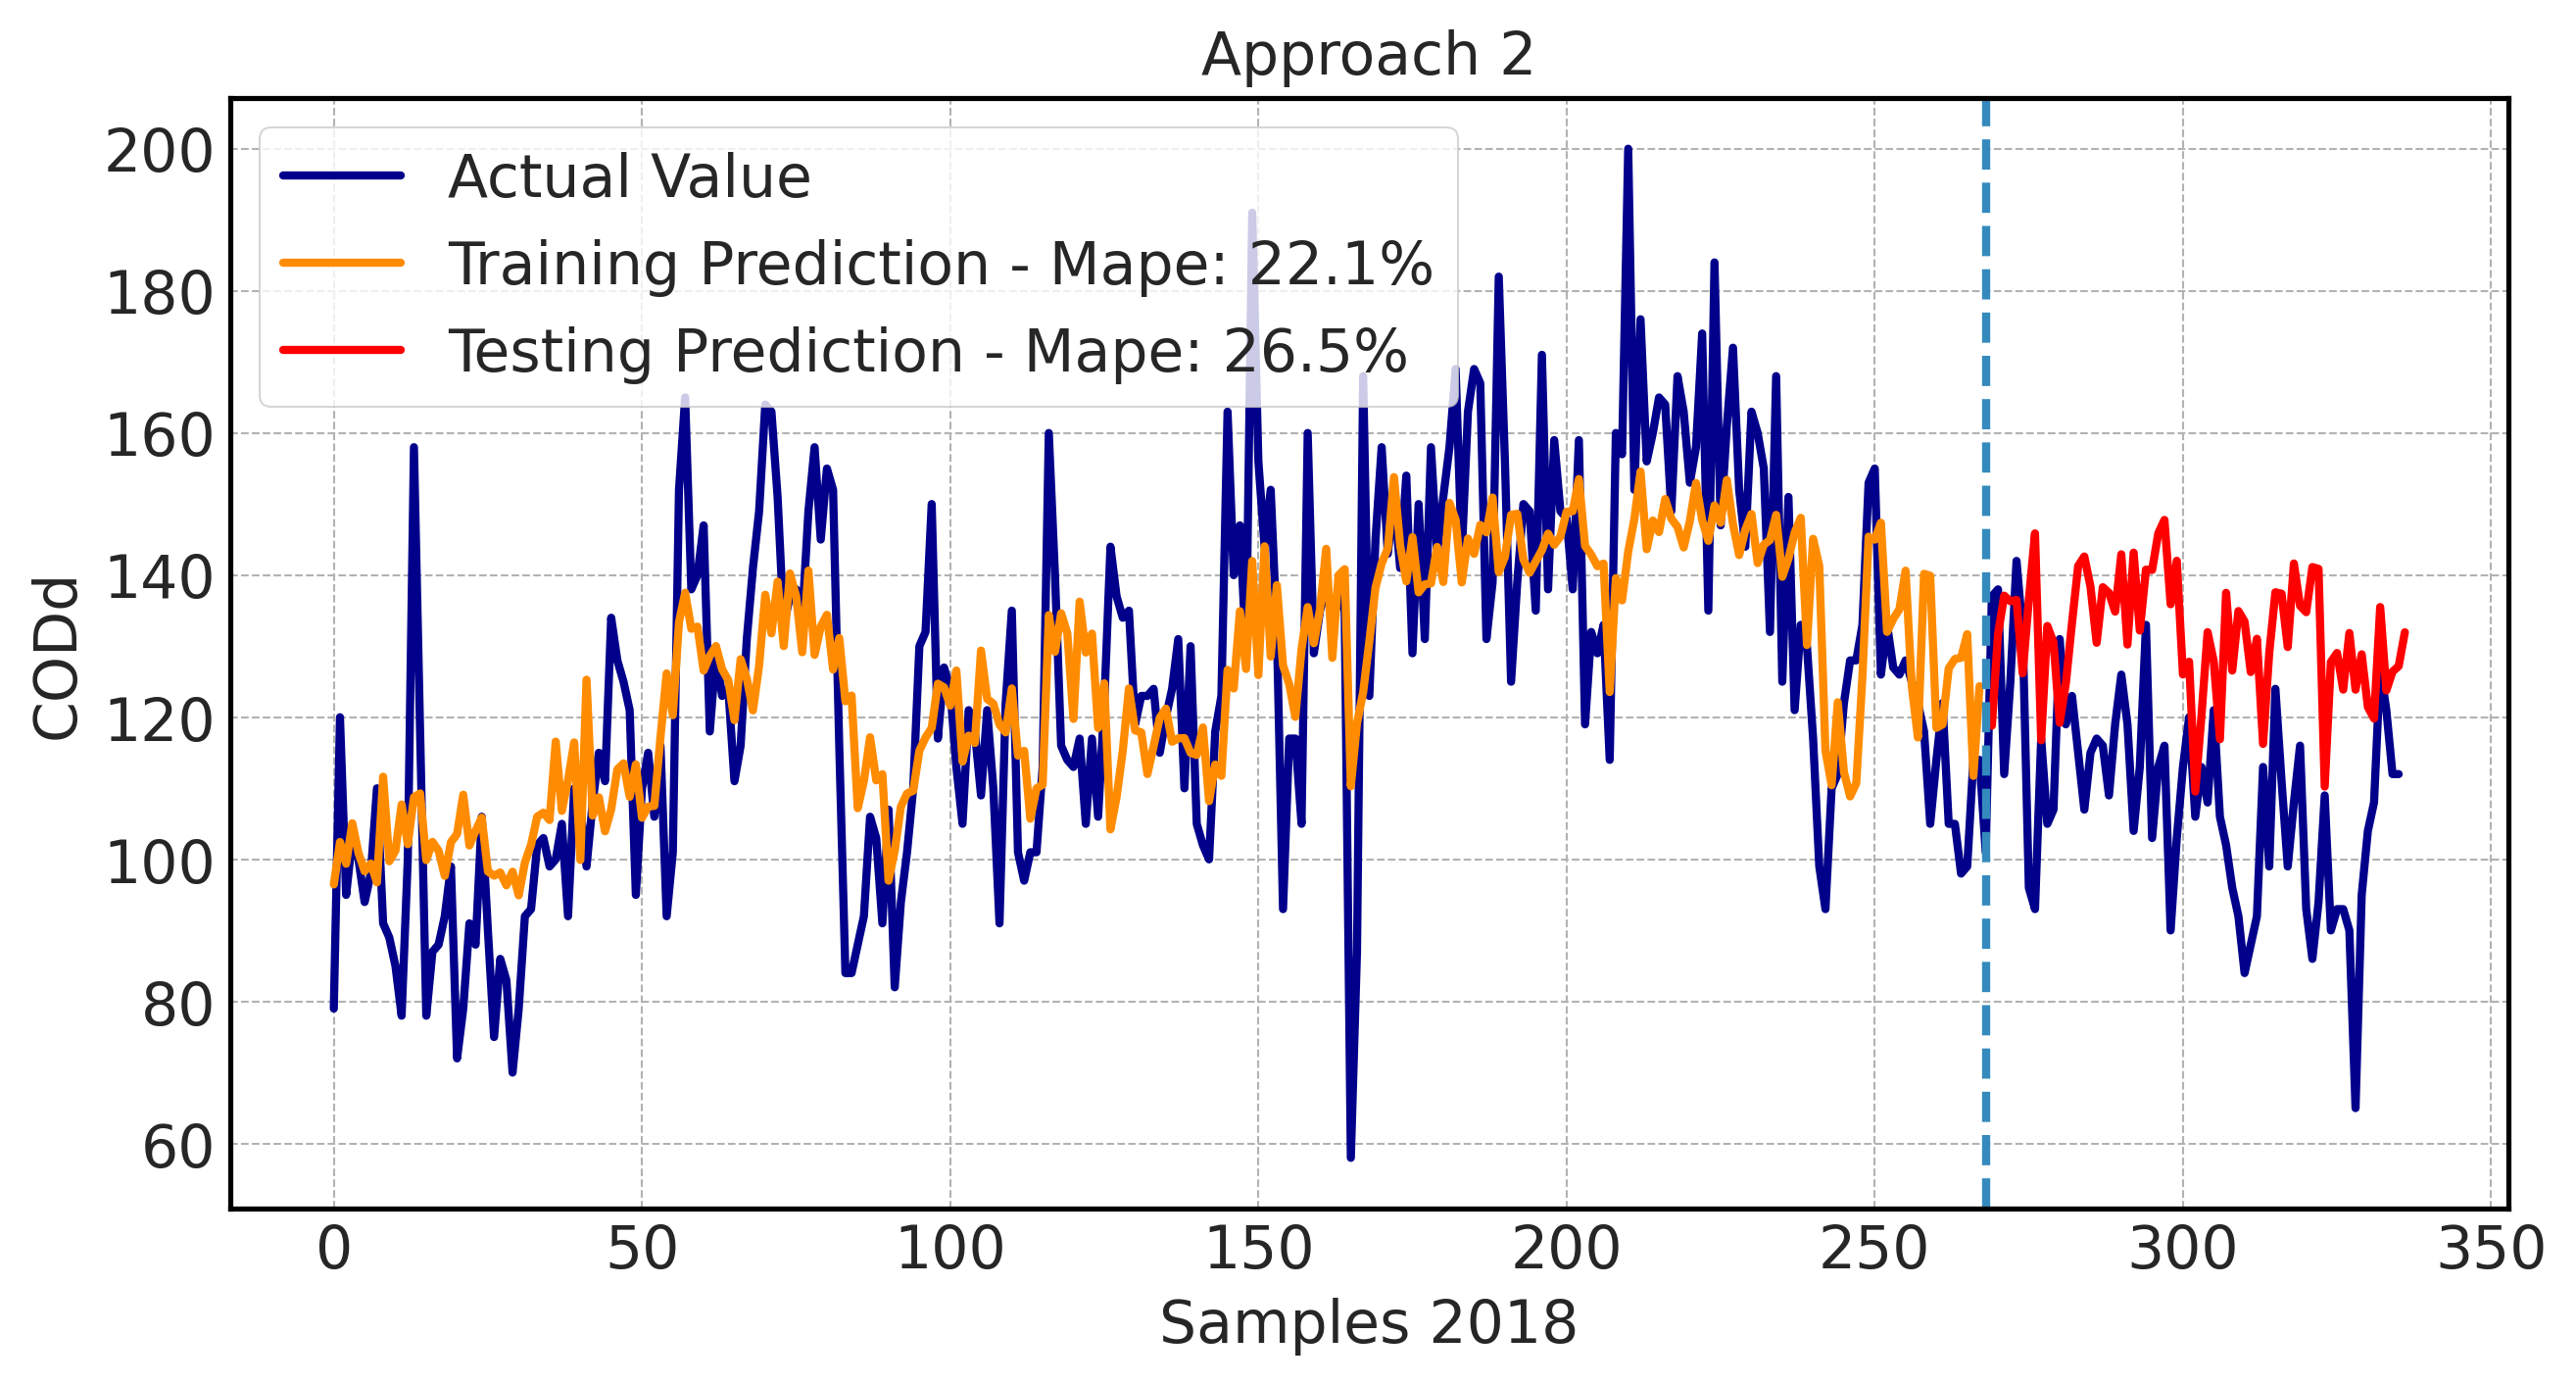
\includegraphics[width=\linewidth]{figures/Ch6/CODd-2.png}
\caption{Approach 2 - CODD}
\label{f:App2-codd}
\end{figure}

\begin{figure}[h]
\centering
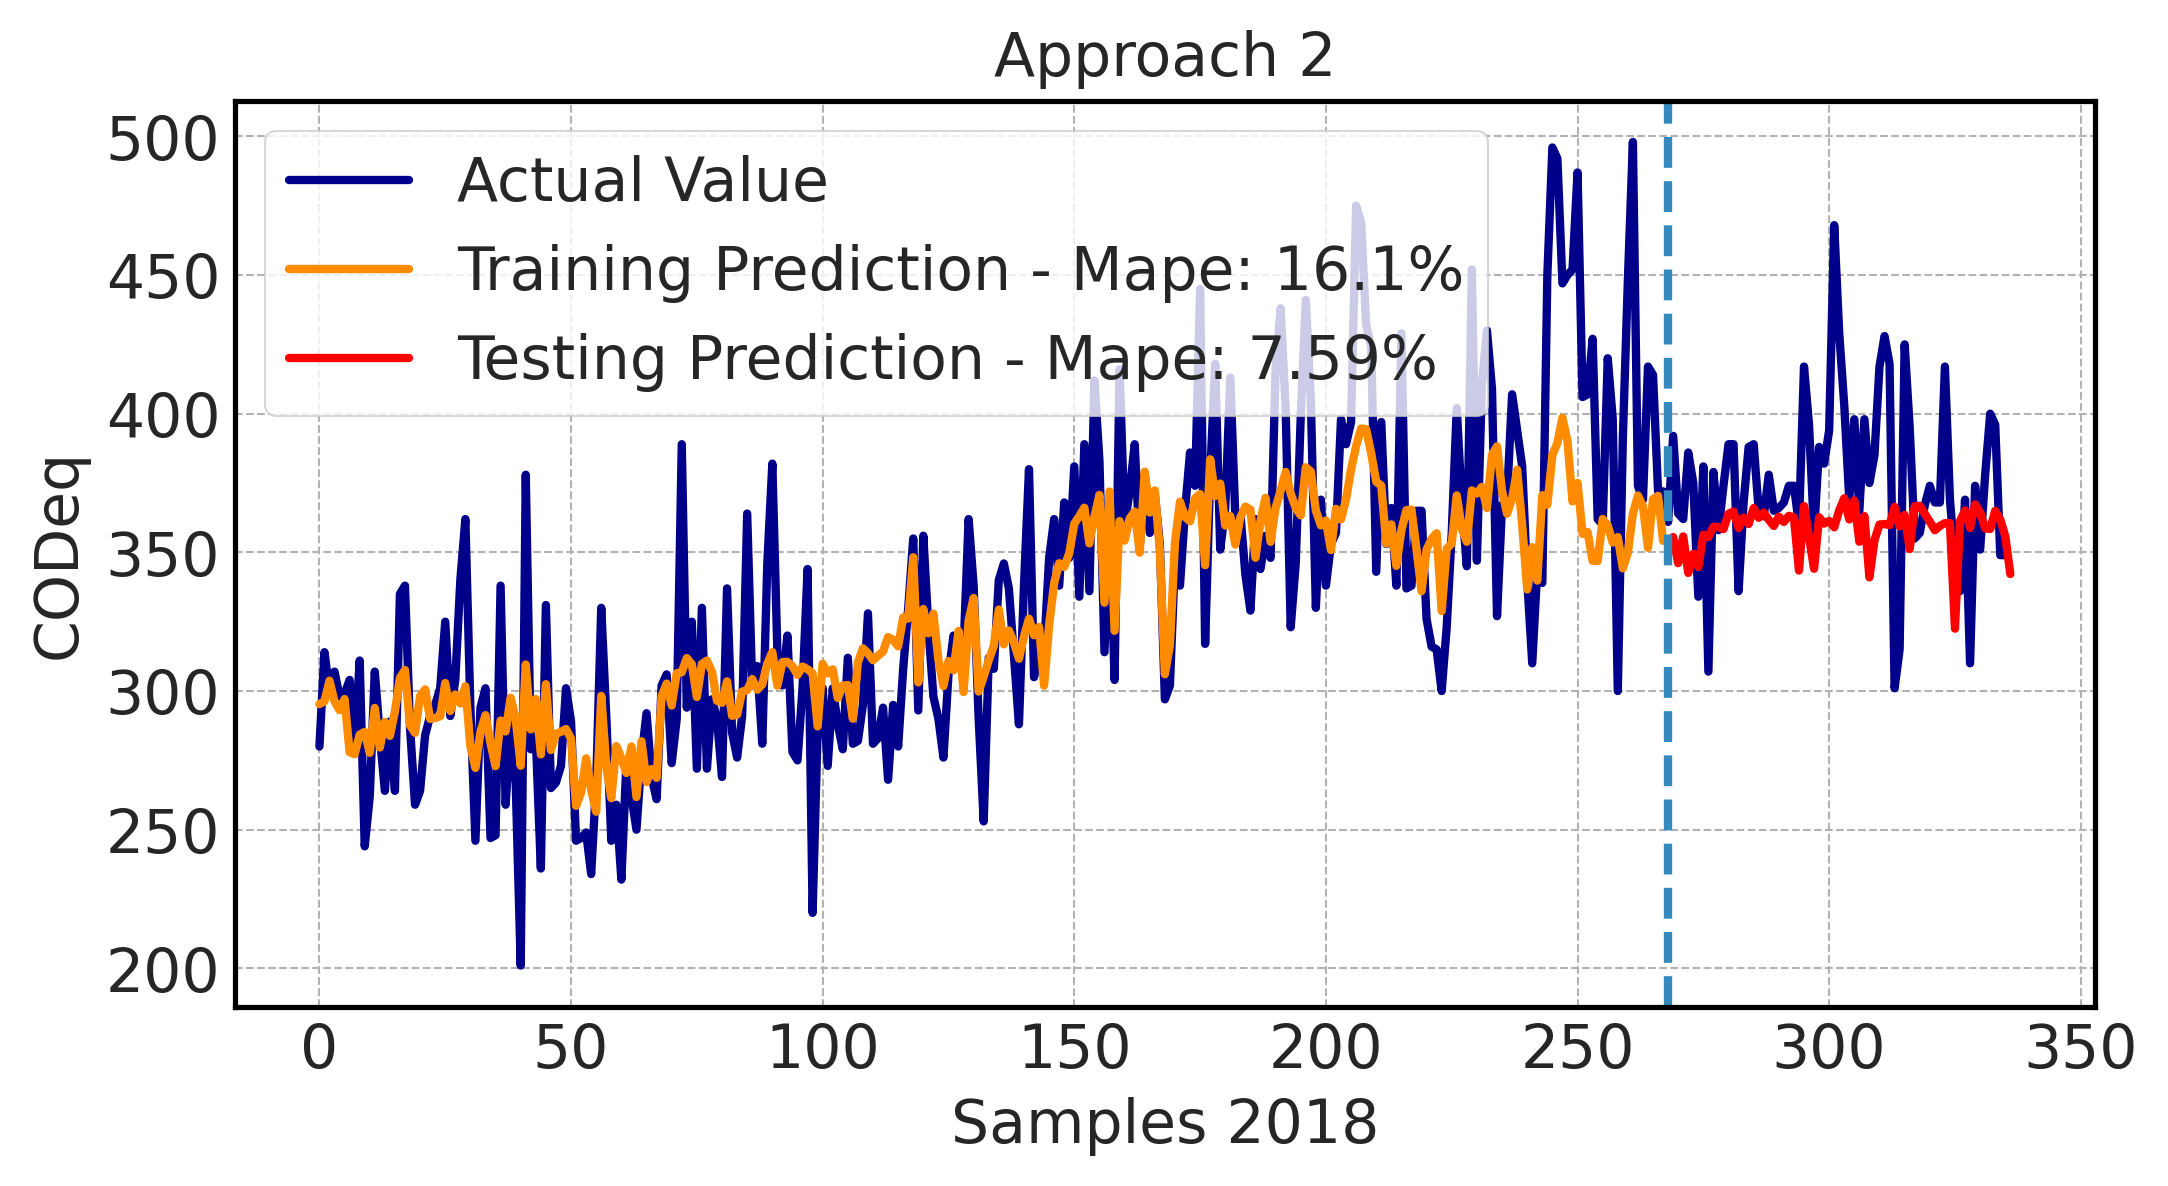
\includegraphics[width=\linewidth]{figures/Ch6/CODeq-2.png}
\caption{Approach 2 - CODEQ}
\label{f:App2-codeq}
\end{figure}

\begin{figure}[h]
\centering
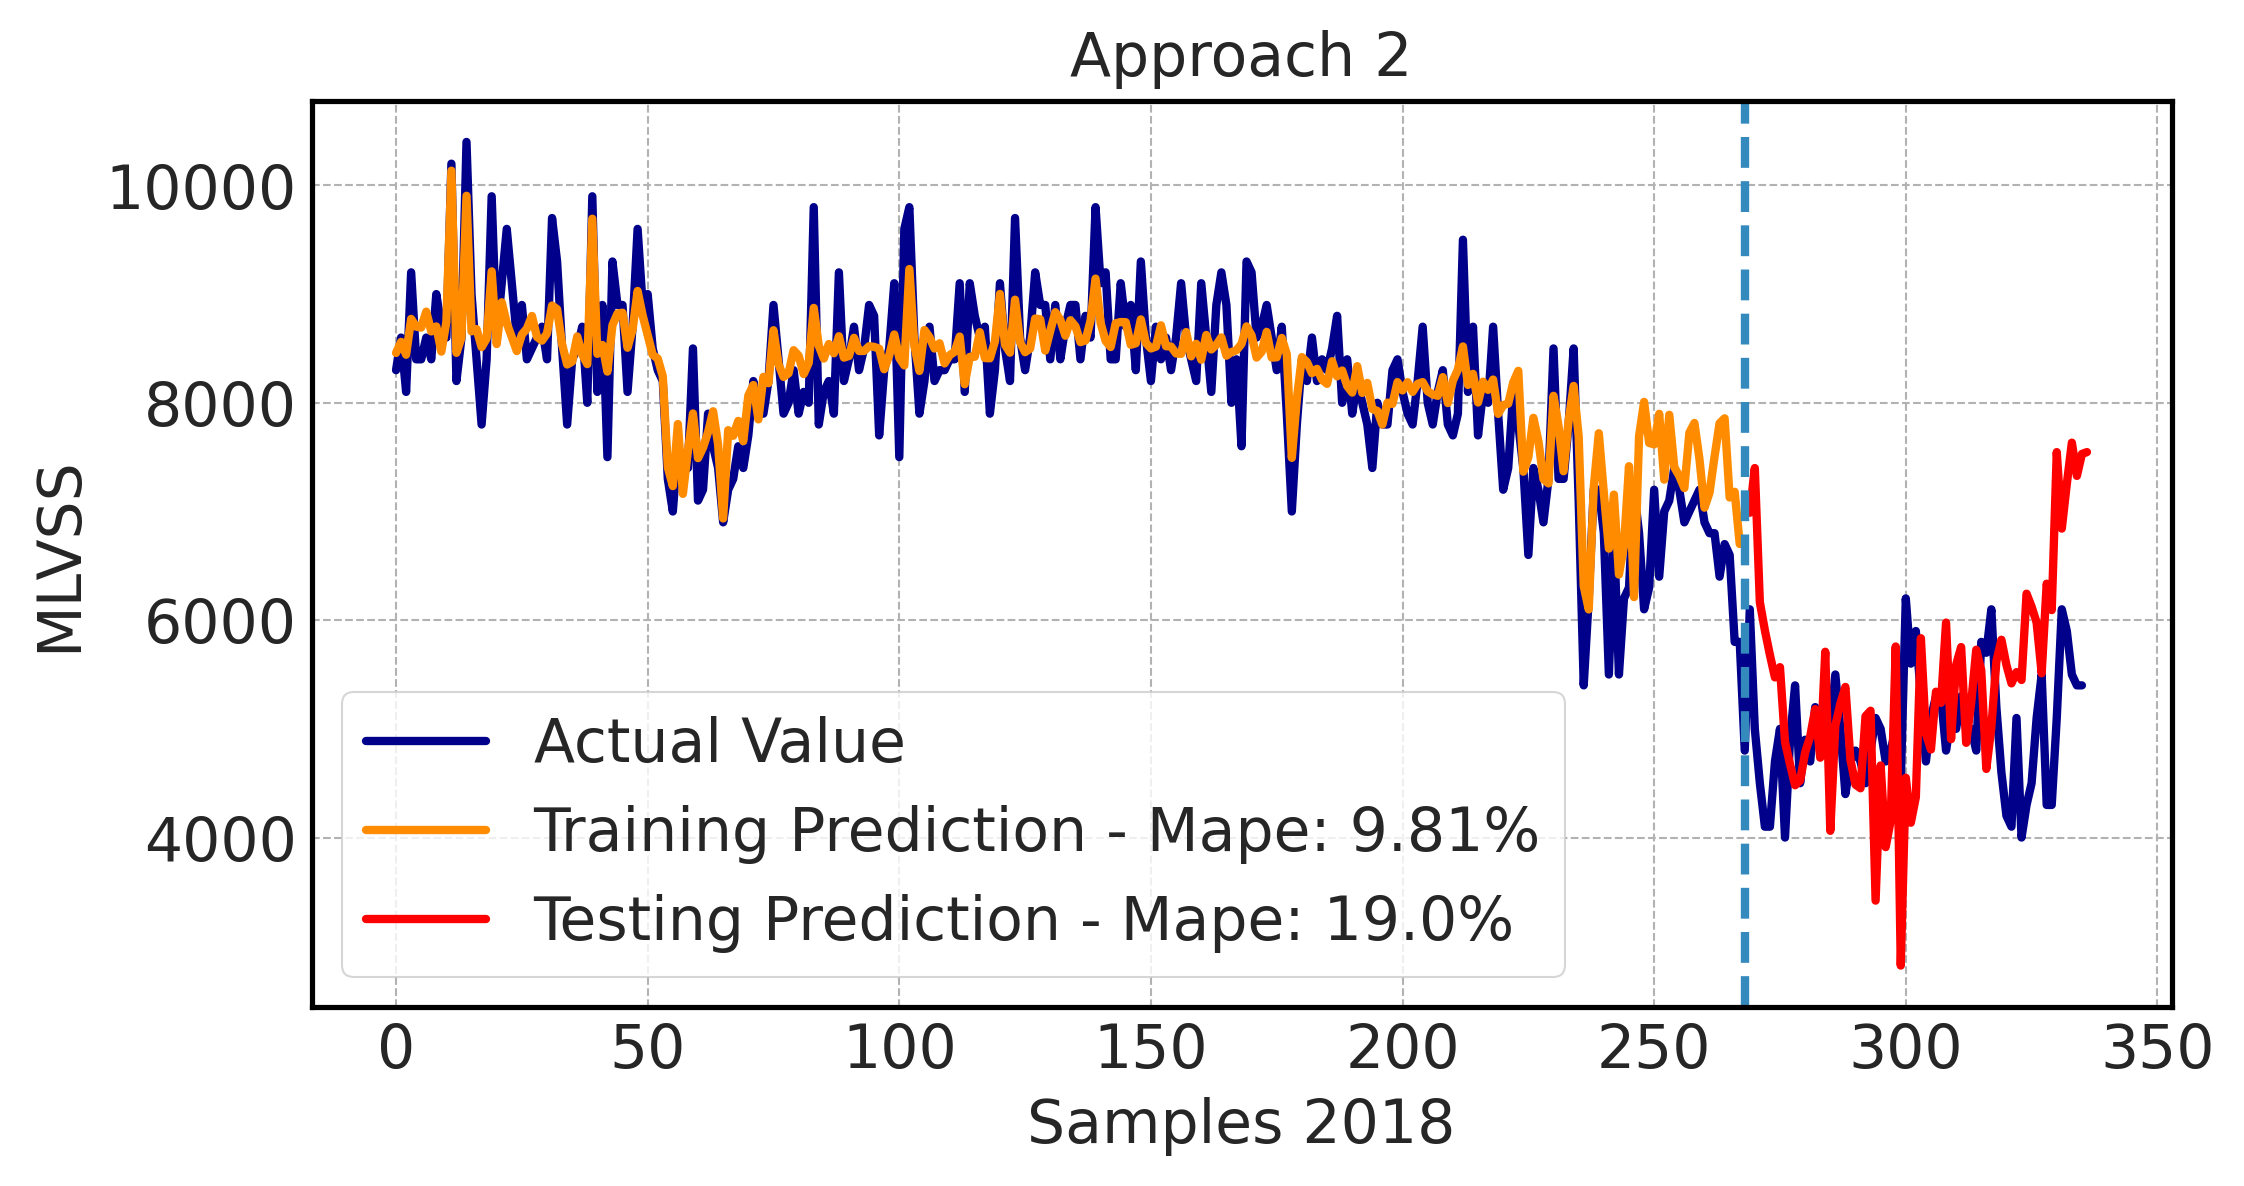
\includegraphics[width=\linewidth]{figures/Ch6/MVLSS-approach2.png}
\caption{Approach 2 - MLVSS}
\label{f:App2-MLVSS}
\end{figure}

\subsection{Minor idea 3}
\label{s:Contribution-2-Major-1-Minor-3}
Develop your idea! For example, explain how the theoretical limits of your approach.

\begin{figure}[h]
\centering
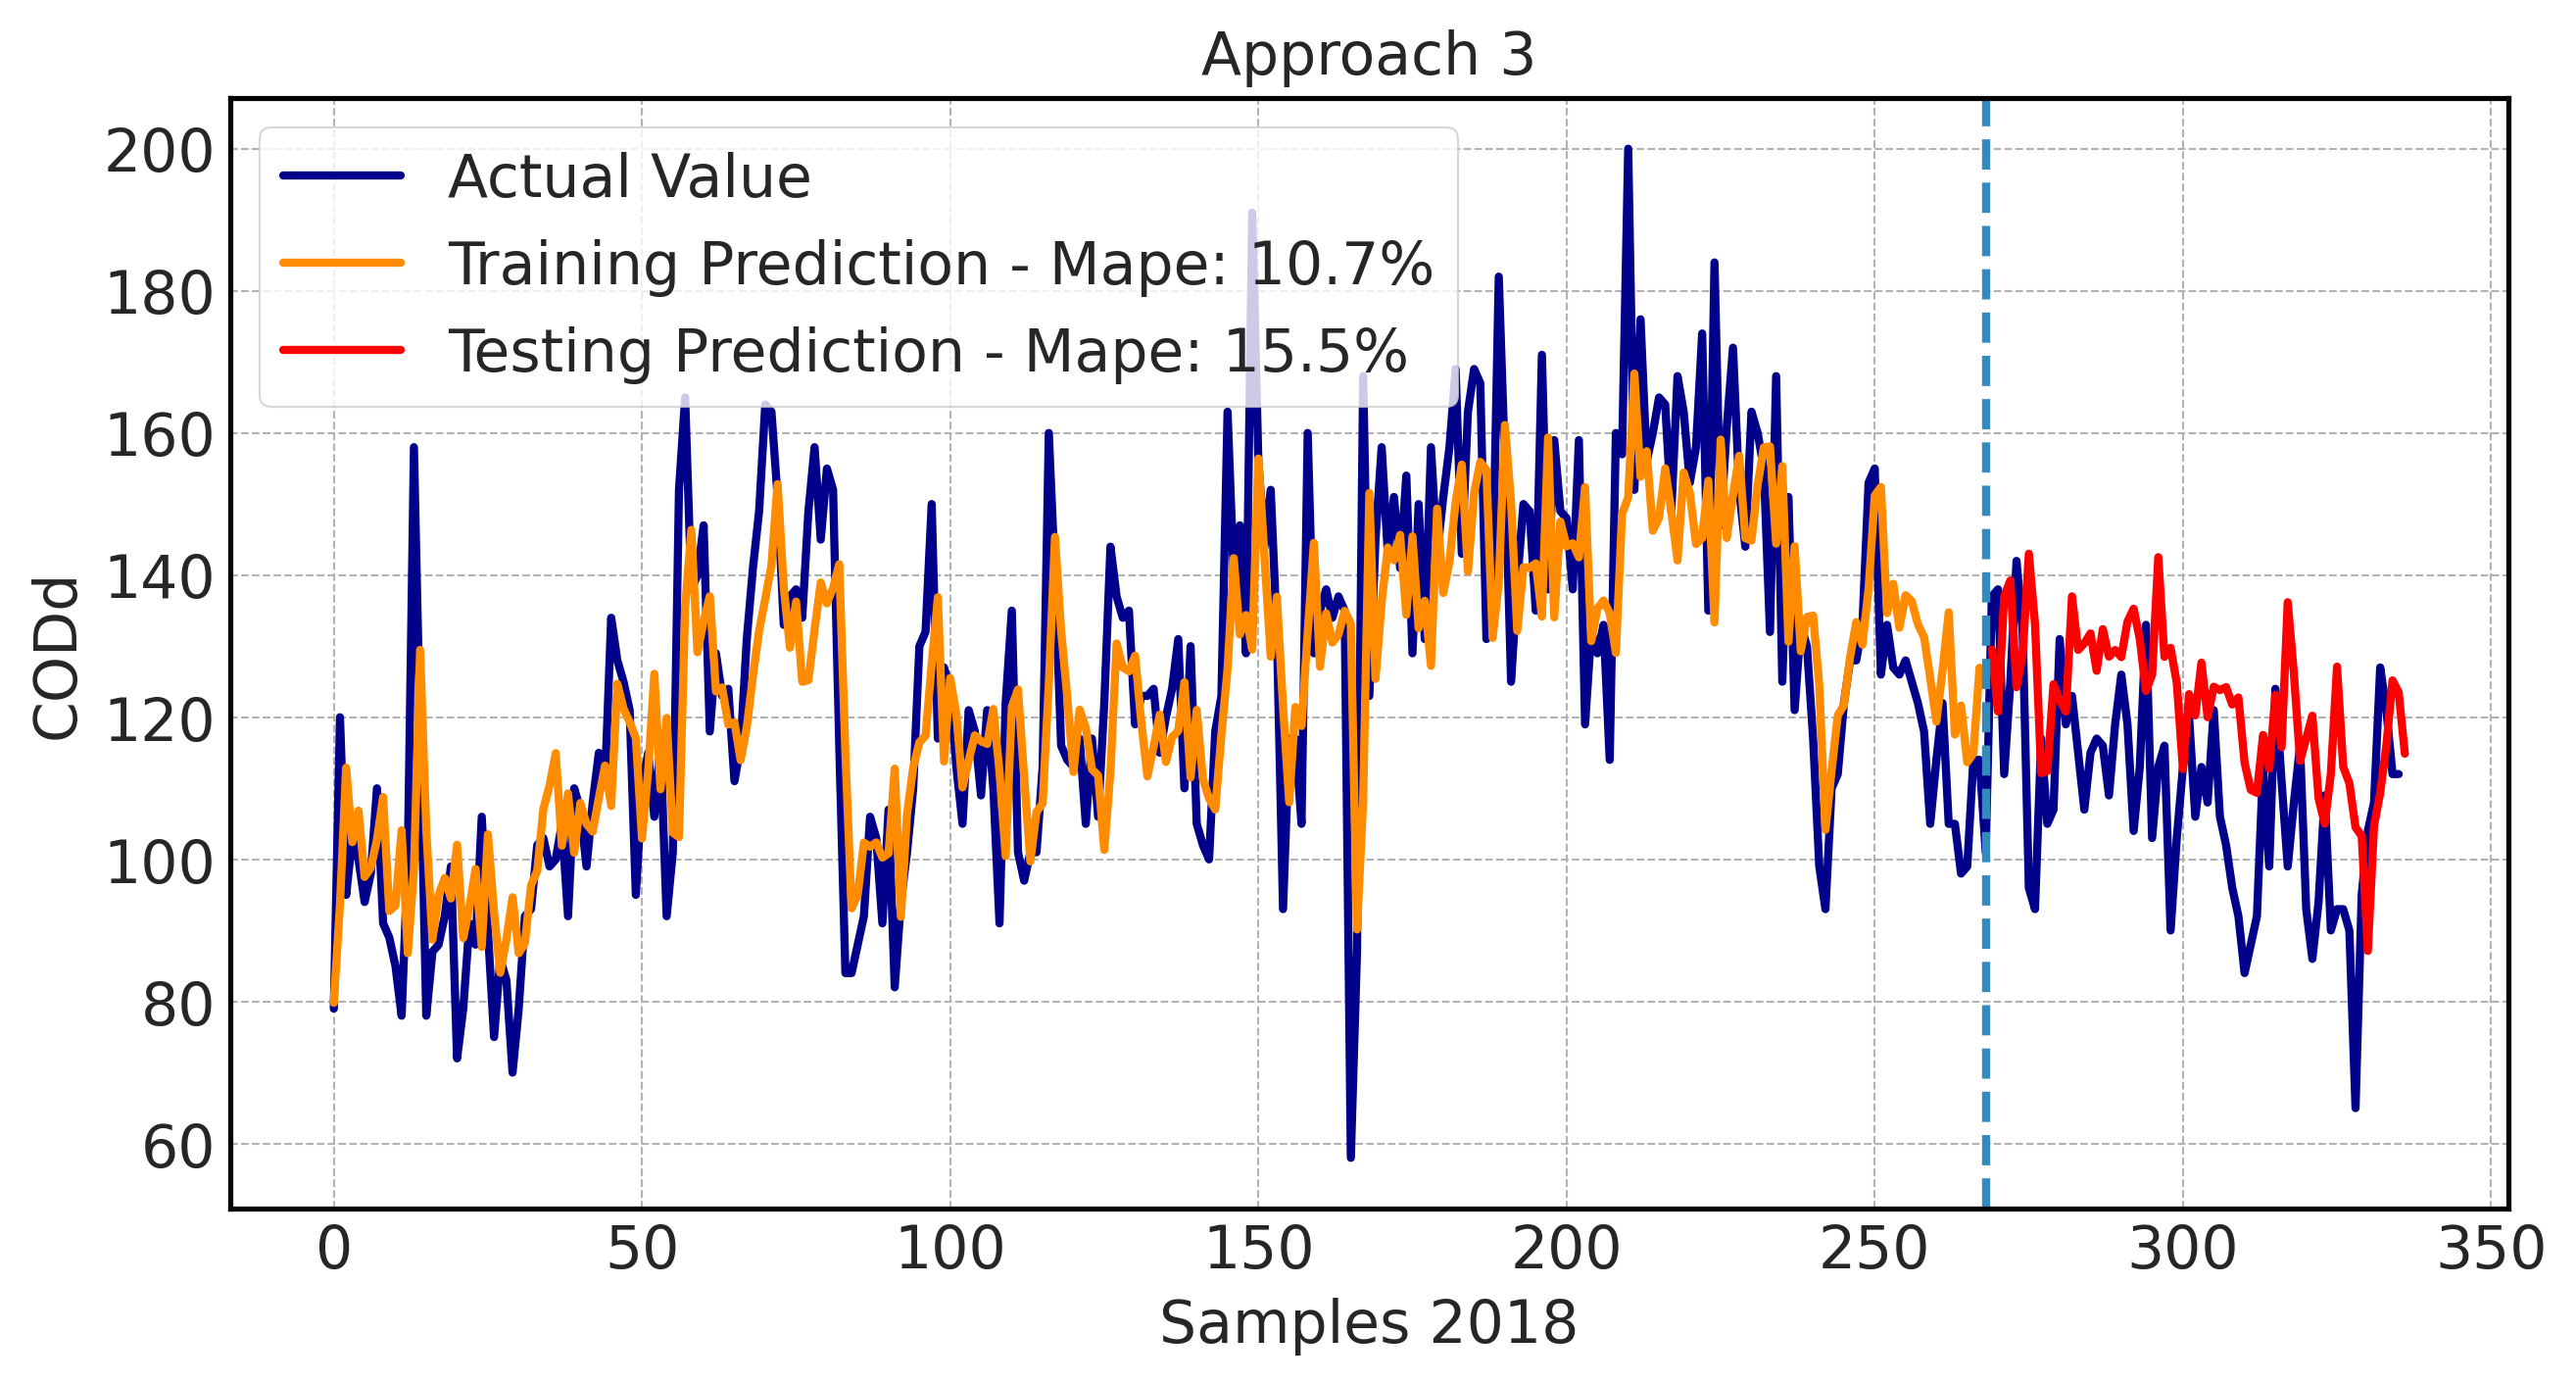
\includegraphics[width=\linewidth]{figures/Ch6/CODd-3.png}
\caption{Approach 3 - CODD}
\label{f:App3-codd}
\end{figure}

\begin{figure}[h]
\centering
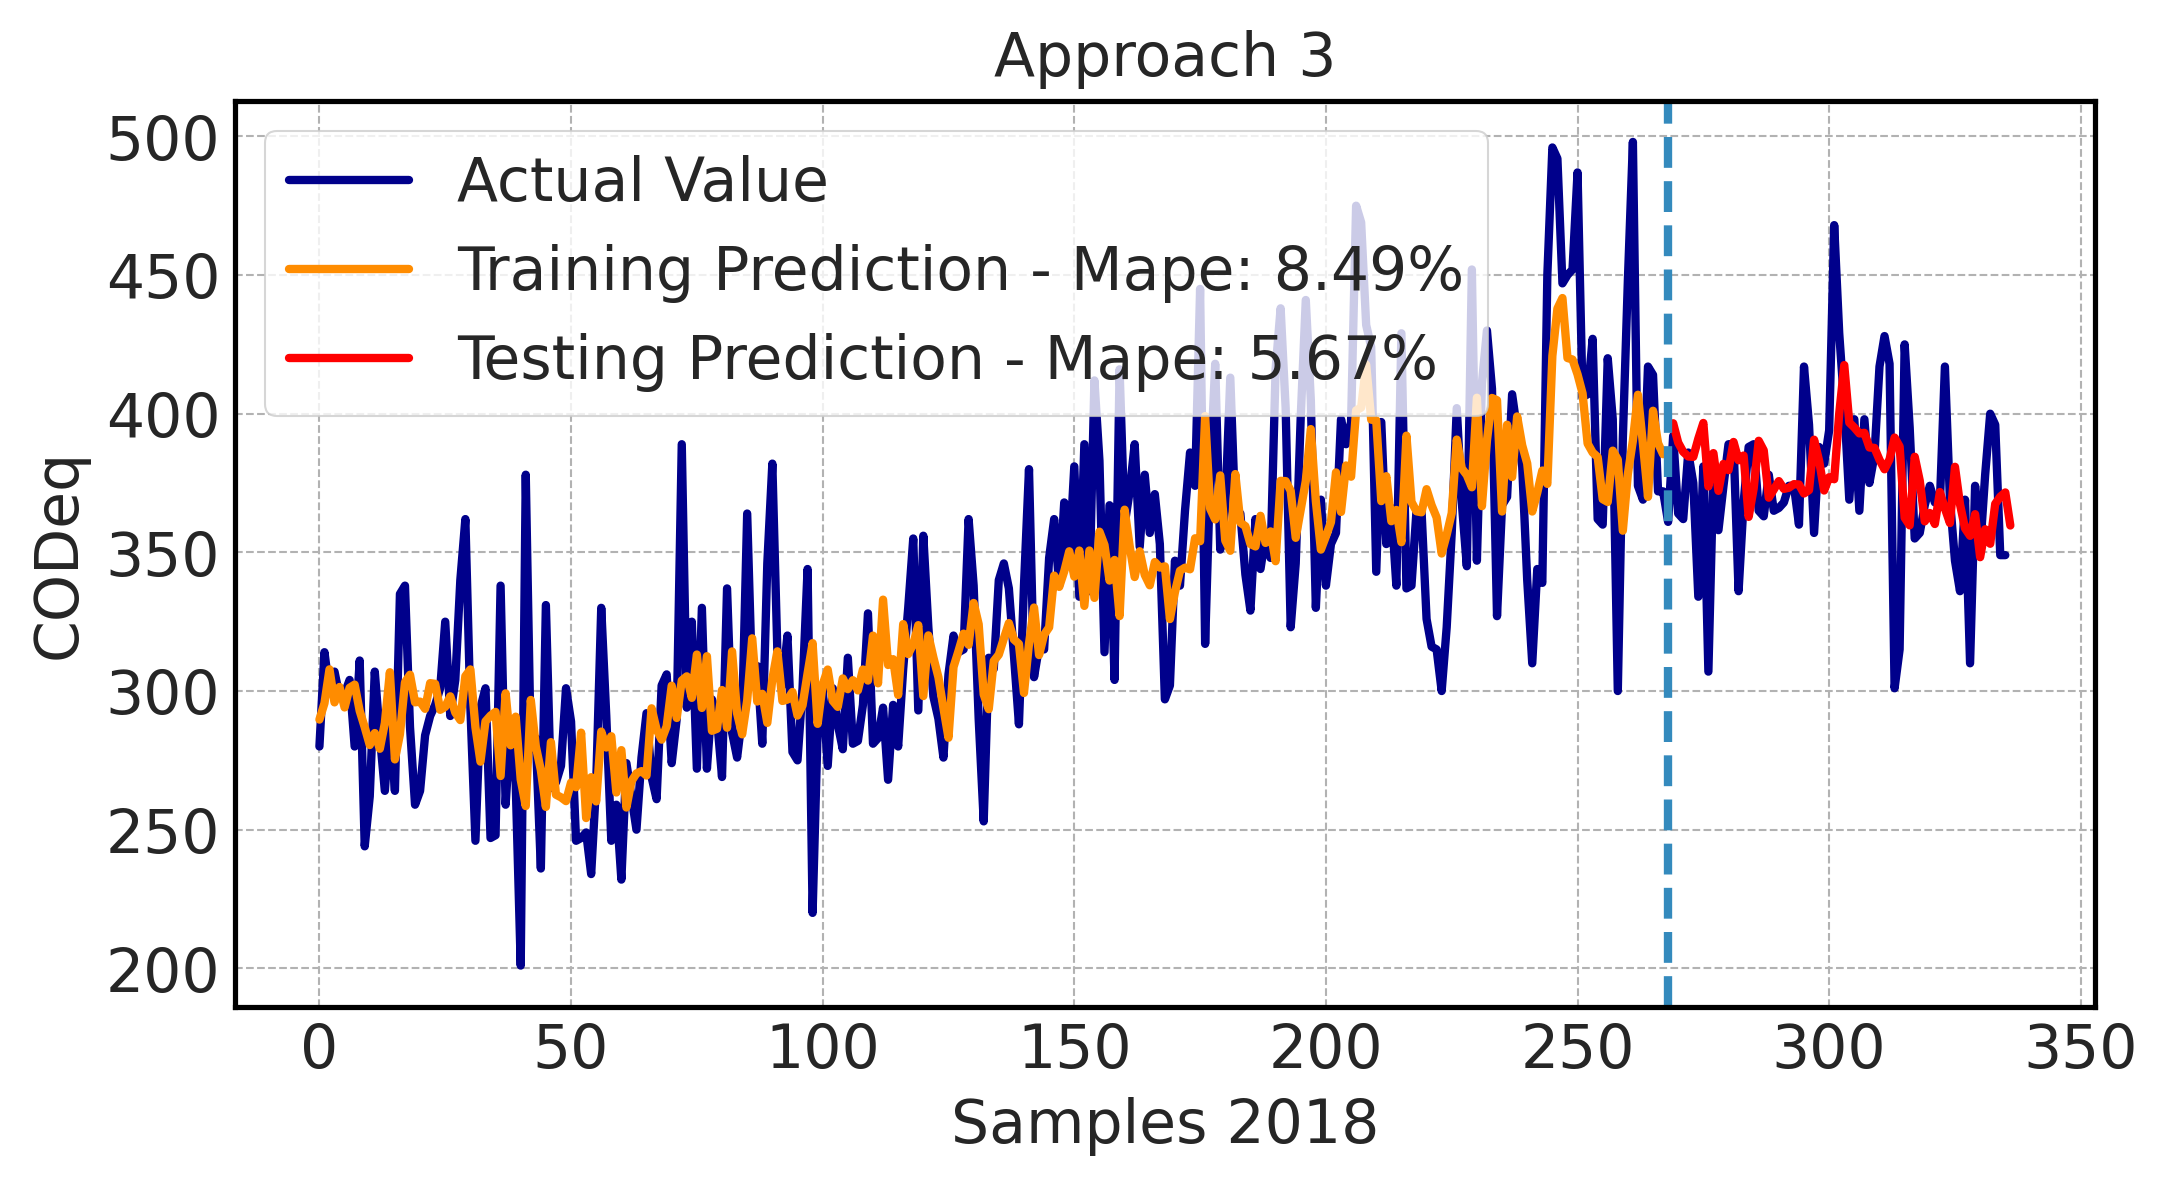
\includegraphics[width=\linewidth]{figures/Ch6/CODeq-3.png}
\caption{Approach 3 - CODEQ}
\label{f:App3-codeq}
\end{figure}

\begin{figure}[h]
\centering
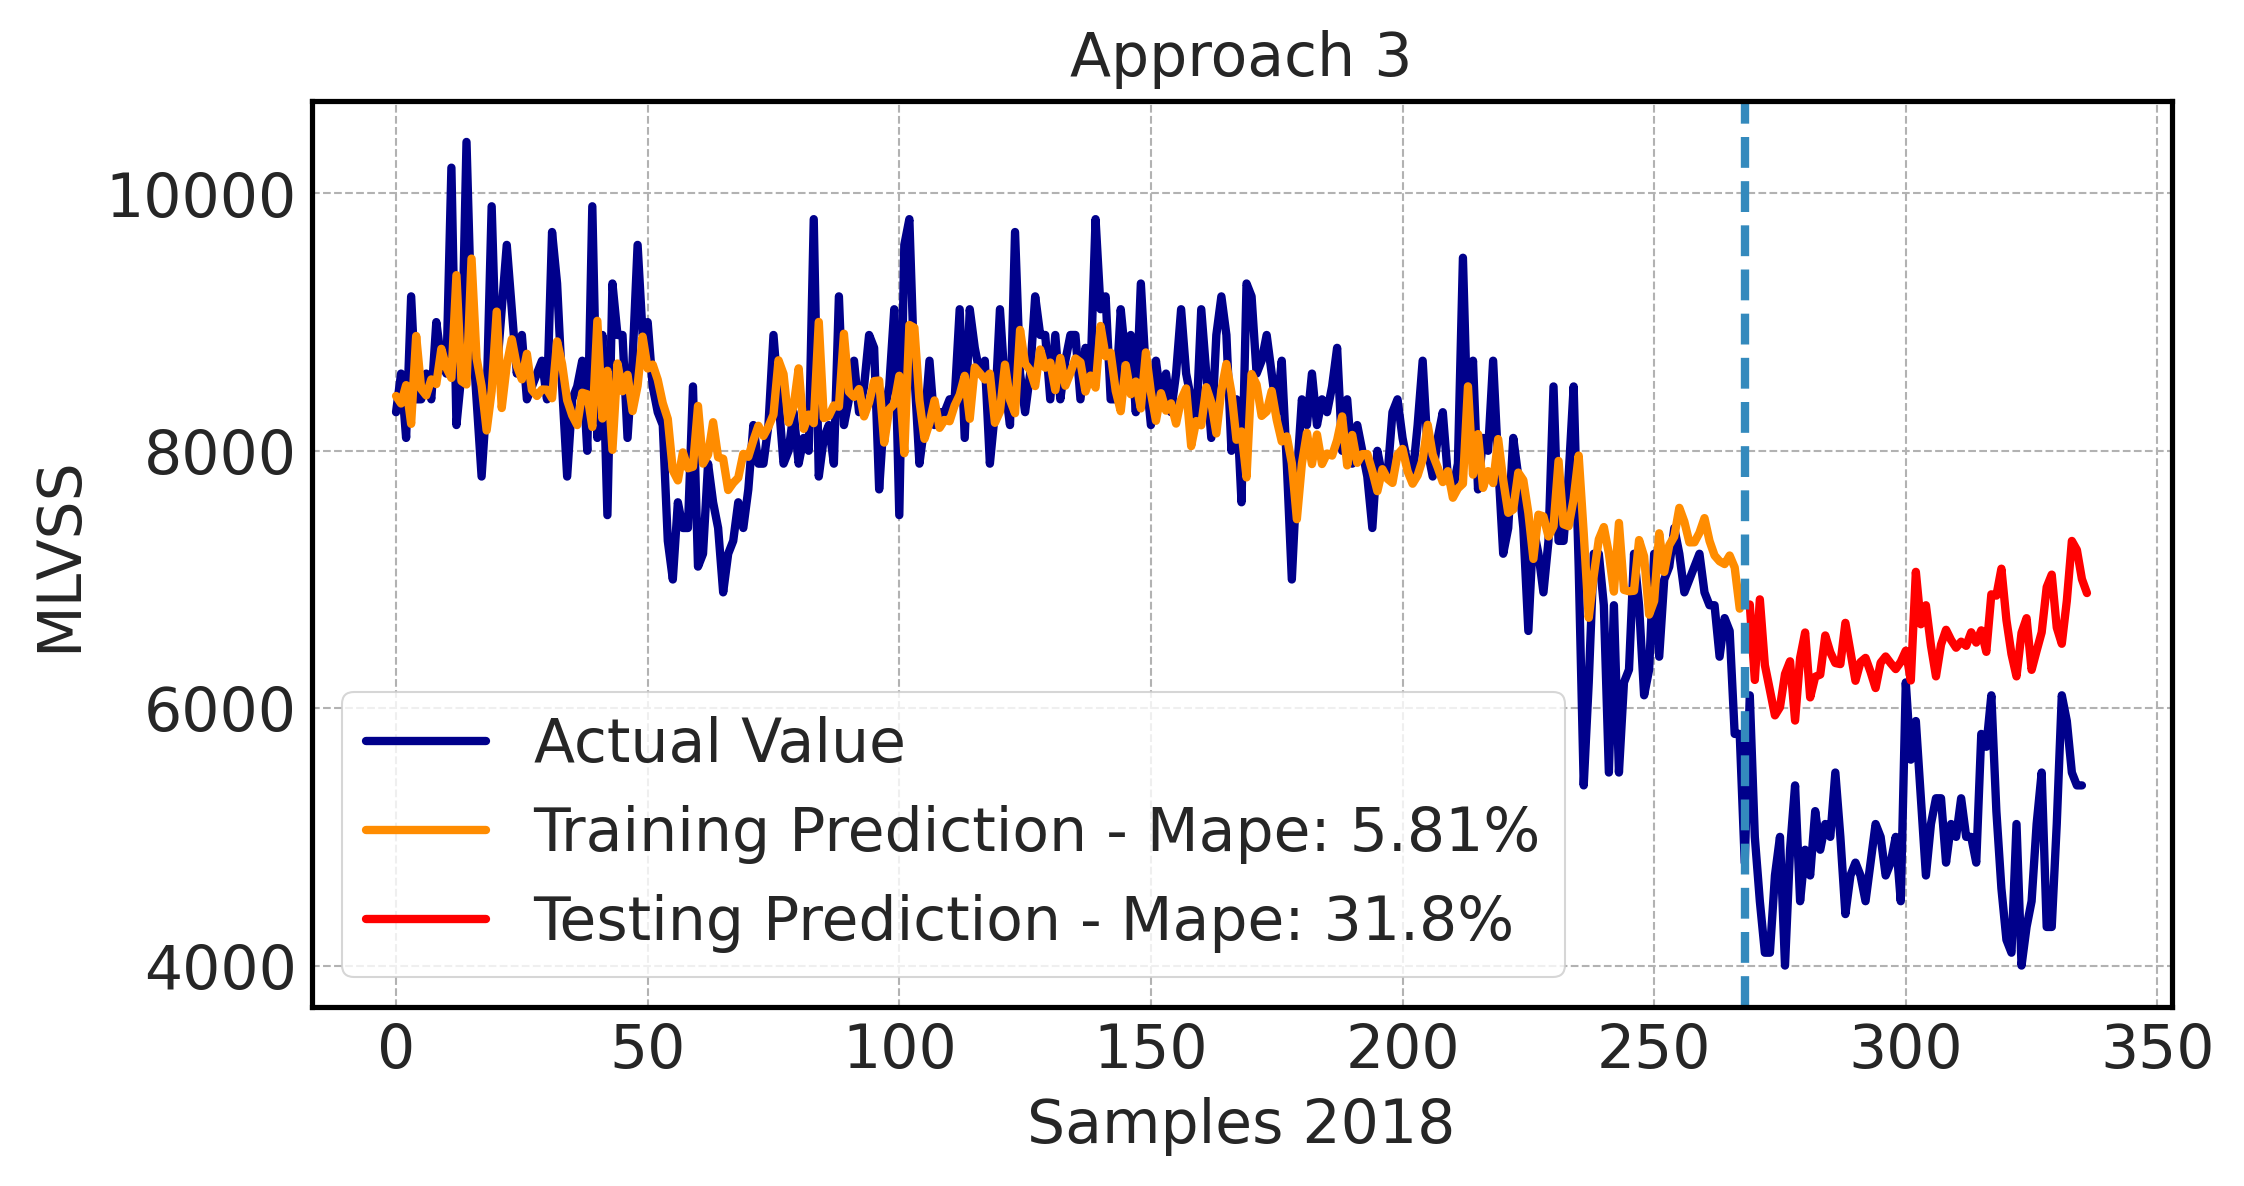
\includegraphics[width=\linewidth]{figures/Ch6/MVLSS-approach3.png}
\caption{Approach 3 - MLVSS}
\label{f:App3-MLVSS}
\end{figure}

\section{Major point 2}
\label{s:Contribution-2-Major-2}
Develop your idea! For example, discuss the difficulties when implementing the proposed algorithm in software.

\subsection{Minor idea 1}
\label{s:Contribution-2-Major-2-Minor-1}
Develop your idea! For example, properties of your implementation.




\subsection{Minor idea 2}
\label{s:Contribution-2-Major-2-Minor-2}
Develop your idea! For example, the particular properties of your implementation.




\section{Summary}
\label{s:Contribution-2-Summary}

Summarize contribution 2. Highlight what makes it relevant. Assuming that the reader knows the details of the contribution now, you should also try to clearly explain in what particular key properties this method deviates from existing research.
